\section{Prompt and Experiment Configuration}
\label{app:prompts}
\paragraph{Common generation contract.}
All seven conditions receive the same assignment, supplied context, requested output constraints, generator model, attempt budget, and information policy. External retrieval is disabled: the coding-agent sandbox denies network access and web search, and conditions are instructed not to introduce facts unsupported by the assignment or supplied context. The Codex wrapper invokes the condition-specific skill and requires the final response to contain the complete generated document rather than a summary or a link to a workspace artifact.

\paragraph{Baseline prompts.}
The single-pass condition begins: ``Write the final response in one generation pass. Do not make a plan for the reader, describe a review, or expose hidden reasoning.'' It then receives the assignment, supplied context, and requested output constraints.

The staged condition uses three fixed prompts. \texttt{Pre-Write} begins: ``Prepare a concise working plan for the next writer. Identify the response's purpose, audience, required content, order, and constraints.'' It explicitly says not to write the final response yet. \texttt{Write} begins: ``Write a complete draft that answers the assignment,'' using the complete \texttt{Pre-Write} output as working guidance. \texttt{Re-Write} begins: ``Revise the draft for instruction fulfillment, organization, depth, audience fit, and factual fidelity.'' Each stage is restricted to the same assignment and supplied context, and the aggregate output-token budget is fixed across the three stages.

The adaptive task-planning condition uses a persistent directed acyclic task graph containing only \texttt{reasoning} and \texttt{composition} nodes. The coordinator recursively decomposes or executes the next dependency-satisfied task and may revise active graph structure after observing composed text. The prompt explicitly forbids adapting by selecting named writing processes; adaptation is restricted to task structure.

\paragraph{Agentic CogWriter and intervention prompts.}
Agentic CogWriter is invoked through the \texttt{agentic-cog-writer} skill. The host agent acts as the \texttt{Monitor}, reads the draft, goal network, and process history, and chooses among \texttt{Planning}, \texttt{Translating}, and \texttt{Reviewing}. The selected process is delegated to the corresponding \texttt{Planner}, \texttt{Translator}, or \texttt{Reviewer} subagent. The skill requires process switches and goal changes to be written to an append-only trace.

The three interventions modify this prompt contract directly. \condNoGoals\ forbids the explicit goal network while retaining adaptive process choice and the three subagents. \condFixedOrder\ preserves the goal network and subagents but replaces adaptive selection with the fixed \texttt{Planning}$\rightarrow$\texttt{Translating}$\rightarrow$\texttt{Reviewing} cycle. \condSingleWriter\ retains adaptive process choice and the goal network but forbids subagent delegation. It also requires each \texttt{Translating} step to append one paragraph before the writer makes the next process decision. Condition configuration files record the skill or stage prompt used for each condition and the SHA-256 hash of fixed stage prompts.

\paragraph{Pairwise judge prompt.}
The primary judge is instructed to act as an impartial judge comparing two responses to the same assignment. Its rubric covers instruction fulfillment, organization and global coherence, content adequacy and depth, style, voice and audience fit, factuality, and constraint fidelity. The prompt explicitly instructs the judge to avoid position bias and length bias, to use only the assignment and supplied context, and to choose \texttt{A}, \texttt{B}, or \texttt{tie}. Each pair is shown in both presentation orders; disagreement across the two orders becomes a tie. The judge returns a JSON record containing the winner, short exact evidence quotes from each response, and a brief rubric-grounded comparison.


\section{Runtime Configuration}
\label{app:runtime}
Table~\ref{tab:runtime-settings} reports the runtime controls shared across conditions.
We hold the generator, output-token budget, network and retrieval policy, approval policy, task input, and final-output requirements fixed so that the compared conditions differ in how they organize the writing process rather than in model access or external information.
Each prompt--condition pair is generated in three runs.
Primary pairwise evaluation uses the same judge for every condition, presents each pair in both orders, and records presentation disagreements as ties; the cross-family judge is used only for the separate robustness analysis.
\begin{table}[H]
\centering
\small
\setlength{\tabcolsep}{5pt}
\begin{tabular}{ll}
\toprule
\textbf{Setting} & \textbf{Value} \\
\midrule
Generator & \modelGen \\
Primary pairwise judge & \modelJudge \\
Cross-family judge & \modelCross \\
Generation runs & 3 per prompt--condition pair \\
Generator output-token budget & 64,000 \\
Generator temperature & unset \\
Network access & denied \\
Web search & disabled \\
Approval policy & never \\
External retrieval & disabled for all conditions \\
Primary judge seed & 20260908 \\
Primary judge retries & 2 \\
Pairwise presentation & both orders \\
Presentation disagreement & counted as tie \\
\bottomrule
\end{tabular}
\caption{Runtime and evaluation settings used for the reported experiments. Model names include the configured reasoning-effort label where applicable.}
\label{tab:runtime-settings}
\end{table}


\section{Generation-Run-Level Pairwise Outcomes}
\label{app:pairwise-detail}
The following figure shows the prompt-level pairwise estimates for each benchmark and generation run, including the ablation contrasts.
For \condAgenticCogWriter\ versus \condSinglePass, the descriptive mean win rates across generation runs are \DoLoFourOneRateMean\ on DoLoMiTes, \HelloFourOneRateMean\ on HelloBench, and \WritingFourOneRateMean\ on WritingBench.
\begin{figure}
\centering
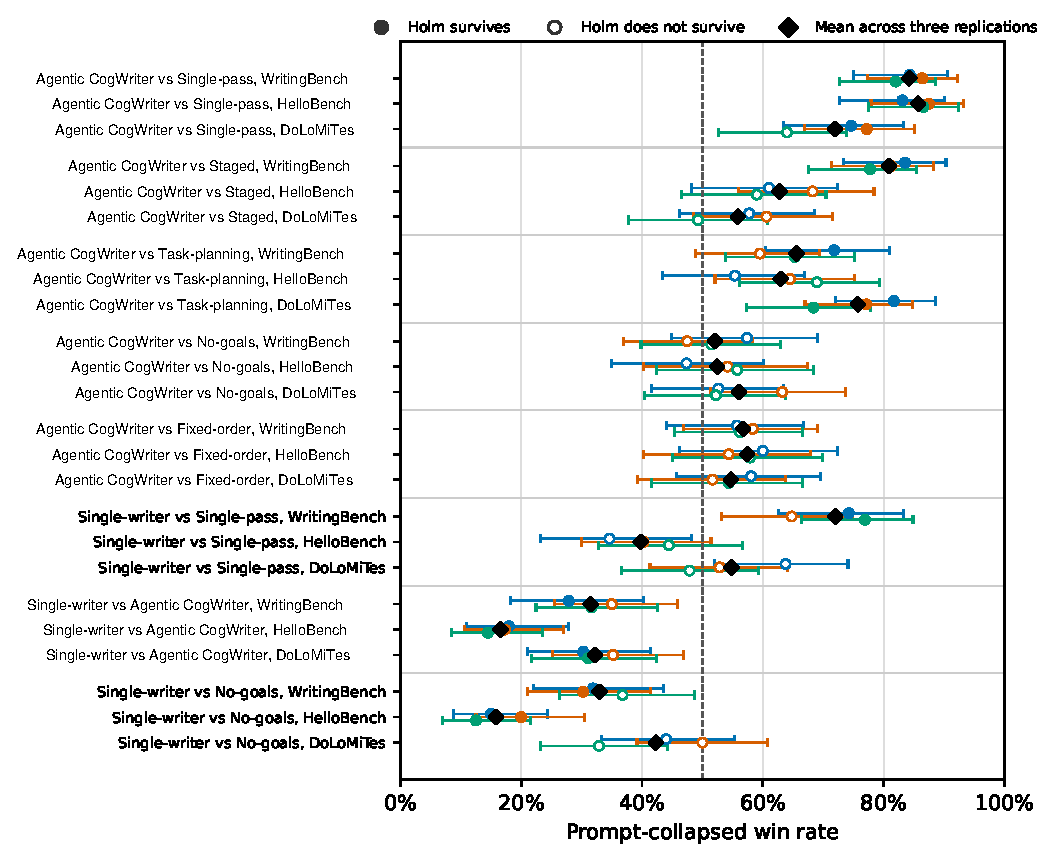
\includegraphics[width=0.96\textwidth]{fig/confirmatory-forest.pdf}
\caption{Run-level pairwise estimates separate the large system comparisons from the ablations.
\condAgenticCogWriter\ is consistently favored over \condSinglePass\ and \condTaskPlanning\ and usually over \condStaged, whereas \condNoGoals\ and \condFixedOrder\ remain near parity and do not survive the within-benchmark Holm correction.
Points show 95\% Wilson intervals; filled circles survive correction, open circles do not, and diamonds are descriptive means across generation runs.}
\label{fig:appendix-confirmatory-forest}
\end{figure}

\section{Paired Document-Quality Differences}
\label{app:paired-quality}
Table~\ref{tab:paired-quality} reports paired differences behind Table~\ref{tab:main-results}
Each prompt's three generation runs are averaged per system before differencing, so the prompt is the resampling unit, and the intervals come from 10,000 prompt-level bootstrap resamples.
\begin{table*}[t]
\centering
\footnotesize
\setlength{\tabcolsep}{2pt}
\begin{tabular}{lrrrrr}
\toprule
& \multicolumn{2}{c}{\textbf{WritingBench}} & \multicolumn{2}{c}{\textbf{HelloBench}} & \textbf{DoLoMiTes} \\
\cmidrule(lr){2-3}\cmidrule(lr){4-5}\cmidrule(lr){6-6}
\textbf{vs.} & \textbf{Native} & \textbf{Pointwise} & \textbf{Native} & \textbf{Pointwise} & \textbf{Pointwise} \\
\midrule
\condSinglePass & \PairedQualityWritingNativeSinglePassDiff\,{\scriptsize[\PairedQualityWritingNativeSinglePassLow, \PairedQualityWritingNativeSinglePassHigh]} & \PairedQualityWritingPointwiseSinglePassDiff\,{\scriptsize[\PairedQualityWritingPointwiseSinglePassLow, \PairedQualityWritingPointwiseSinglePassHigh]} & \PairedQualityHelloNativeSinglePassDiff\,{\scriptsize[\PairedQualityHelloNativeSinglePassLow, \PairedQualityHelloNativeSinglePassHigh]} & \PairedQualityHelloPointwiseSinglePassDiff\,{\scriptsize[\PairedQualityHelloPointwiseSinglePassLow, \PairedQualityHelloPointwiseSinglePassHigh]} & \PairedQualityDoLoPointwiseSinglePassDiff\,{\scriptsize[\PairedQualityDoLoPointwiseSinglePassLow, \PairedQualityDoLoPointwiseSinglePassHigh]} \\
\condStaged & \PairedQualityWritingNativeStagedDiff\,{\scriptsize[\PairedQualityWritingNativeStagedLow, \PairedQualityWritingNativeStagedHigh]} & \PairedQualityWritingPointwiseStagedDiff\,{\scriptsize[\PairedQualityWritingPointwiseStagedLow, \PairedQualityWritingPointwiseStagedHigh]} & \PairedQualityHelloNativeStagedDiff\,{\scriptsize[\PairedQualityHelloNativeStagedLow, \PairedQualityHelloNativeStagedHigh]} & \PairedQualityHelloPointwiseStagedDiff\,{\scriptsize[\PairedQualityHelloPointwiseStagedLow, \PairedQualityHelloPointwiseStagedHigh]} & \PairedQualityDoLoPointwiseStagedDiff\,{\scriptsize[\PairedQualityDoLoPointwiseStagedLow, \PairedQualityDoLoPointwiseStagedHigh]} \\
\condTaskPlanning & \PairedQualityWritingNativeTaskPlanningDiff\,{\scriptsize[\PairedQualityWritingNativeTaskPlanningLow, \PairedQualityWritingNativeTaskPlanningHigh]} & \PairedQualityWritingPointwiseTaskPlanningDiff\,{\scriptsize[\PairedQualityWritingPointwiseTaskPlanningLow, \PairedQualityWritingPointwiseTaskPlanningHigh]} & \PairedQualityHelloNativeTaskPlanningDiff\,{\scriptsize[\PairedQualityHelloNativeTaskPlanningLow, \PairedQualityHelloNativeTaskPlanningHigh]} & \PairedQualityHelloPointwiseTaskPlanningDiff\,{\scriptsize[\PairedQualityHelloPointwiseTaskPlanningLow, \PairedQualityHelloPointwiseTaskPlanningHigh]} & \PairedQualityDoLoPointwiseTaskPlanningDiff\,{\scriptsize[\PairedQualityDoLoPointwiseTaskPlanningLow, \PairedQualityDoLoPointwiseTaskPlanningHigh]} \\
\bottomrule
\end{tabular}
\caption{Paired differences in document quality, \condAgenticCogWriter\ minus the compared system, with 95\% bootstrap intervals in brackets. Each prompt's three generation runs are averaged per system before differencing, and prompts are resampled 10,000 times; positive values favor \condAgenticCogWriter, and intervals that exclude zero indicate a difference beyond prompt-level sampling variation.}
\label{tab:paired-quality}
\end{table*}


\section{Additional Process and Resource Statistics}
\label{app:process-behavior}
Table~\ref{tab:process-summary} reports completion, output size, delegated invocations, goal events, token accounting, and wall-clock time from the first generation run.
For \condAgenticCogWriter, that run uses \AfourOutputTokens\ output-plus-reasoning tokens and \AfourInputTokens\ uncached input tokens per attempted run and records \AfourGoalRegenerated\ accepted goal regeneration.
Across the three generation runs, the trace summaries contain mean totals of \AfourGoalCreatedMean\ goal-creation events and \AfourGoalDevelopedMean\ goal-development events, while the post-\texttt{Reviewing} ledger contains \AfourLedgerEntriesMean\ entries including \AfourLedgerWithProposalMean\ explicit regeneration proposals.
\begin{table}[H]
\centering
\small
\setlength{\tabcolsep}{4pt}
\begin{tabular}{lrrrrrr}
\toprule
\textbf{Condition}
& \shortstack{\textbf{Median}\\\textbf{units}}
& \shortstack{\textbf{Spawns}\\\textbf{/run}}
& \shortstack{\textbf{Goals}\\\textbf{created/developed/regenerated}}
& \shortstack{\textbf{Output}\\\textbf{tokens}\\\textbf{/run}}
& \shortstack{\textbf{Input}\\\textbf{tokens}\\\textbf{/run}}
& \shortstack{\textbf{Mean sec.}\\\textbf{/completed run}} \\
\cmidrule(lr){1-1}\cmidrule(lr){2-2}\cmidrule(lr){3-3}\cmidrule(lr){4-4}\cmidrule(lr){5-5}\cmidrule(lr){6-6}\cmidrule(lr){7-7}
\condSinglePass & \AoneMedianOutputMean & \AoneSpawnsMean & \AoneGoalCreatedMean/\AoneGoalDevelopedMean/\AoneGoalRegeneratedMean & \AoneOutputTokensMean & \AoneInputTokensMean & \AoneMeanSecondsMean \\
\condStaged & \AtwoMedianOutputMean & \AtwoSpawnsMean & \AtwoGoalCreatedMean/\AtwoGoalDevelopedMean/\AtwoGoalRegeneratedMean & \AtwoOutputTokensMean & \AtwoInputTokensMean & \AtwoMeanSecondsMean \\
\condTaskPlanning & \AthreeMedianOutputMean & \AthreeSpawnsMean & \AthreeGoalCreatedMean/\AthreeGoalDevelopedMean/\AthreeGoalRegeneratedMean & \AthreeOutputTokensMean & \AthreeInputTokensMean & \AthreeMeanSecondsMean \\
\rowcolor{black!5}
\condAgenticCogWriter & \AfourMedianOutputMean & \AfourSpawnsMean & \AfourGoalCreatedMean/\AfourGoalDevelopedMean/\AfourGoalRegeneratedMean & \AfourOutputTokensMean & \AfourInputTokensMean & \AfourMeanSecondsMean \\
\condNoGoals & \AfiveMedianOutputMean & \AfiveSpawnsMean & \AfiveGoalCreatedMean/\AfiveGoalDevelopedMean/\AfiveGoalRegeneratedMean & \AfiveOutputTokensMean & \AfiveInputTokensMean & \AfiveMeanSecondsMean \\
\condFixedOrder & \AsixMedianOutputMean & \AsixSpawnsMean & \AsixGoalCreatedMean/\AsixGoalDevelopedMean/\AsixGoalRegeneratedMean & \AsixOutputTokensMean & \AsixInputTokensMean & \AsixMeanSecondsMean \\
\condSingleWriter & \AsevenMedianOutputMean & \AsevenSpawnsMean & \AsevenGoalCreatedMean/\AsevenGoalDevelopedMean/\AsevenGoalRegeneratedMean & \AsevenOutputTokensMean & \AsevenInputTokensMean & \AsevenMeanSecondsMean \\
\bottomrule
\end{tabular}
\caption{Process and resource use across the three generation runs. Each value is the mean of the three run-level summaries; Median units therefore averages the run-level medians rather than recomputing a median after joining runs. Goal entries report mean created/developed/regenerated events. These realized differences motivate the output-length and compute-matched sensitivity analyses rather than treating raw resource use as a controlled mechanism.}
\label{tab:process-summary}
\end{table}


\section{Sensitivity Analyses}
\label{app:sensitivity-analyses}
\subsection{Record-Pooled Sensitivity}
\label{app:record-pooled}
Table~\ref{tab:appendix-record-pooled-pairwise} reports a sensitivity analysis that treats the two presentation records for each prompt as independent observations; the retained disagreements show how much presentation order can affect the descriptive rates.
The retained presentation disagreements were \WritingPresentationDisagreementRate\ on WritingBench, \HelloPresentationDisagreementRate\ on HelloBench, and \DoLoPresentationDisagreementRate\ on DoLoMiTes across the three generation runs.
\begin{table}[H]
\centering
\small
\setlength{\tabcolsep}{3pt}
\begin{tabular}{lcccc}
\toprule
\textbf{Contrast}
& \textbf{WritingBench}
& \textbf{HelloBench}
& \textbf{DoLoMiTes}
& \shortstack{\textbf{Pooled mean (SD);}\\\textbf{Wilson interval, first replication}} \\
\midrule
\condFull\ vs \condSinglePass
& \RecordWritingFourOneRateMean\ (\RecordWritingFourOneRateSD)
& \RecordHelloFourOneRateMean\ (\RecordHelloFourOneRateSD)
& \RecordDoLoFourOneRateMean\ (\RecordDoLoFourOneRateSD)
& \RecordPooledFourOneRateMean\ (\RecordPooledFourOneRateSD); \RecordPooledFourOneInterval \\
\condFull\ vs \condStaged
& \RecordWritingFourTwoRateMean\ (\RecordWritingFourTwoRateSD)
& \RecordHelloFourTwoRateMean\ (\RecordHelloFourTwoRateSD)
& \RecordDoLoFourTwoRateMean\ (\RecordDoLoFourTwoRateSD)
& \RecordPooledFourTwoRateMean\ (\RecordPooledFourTwoRateSD); \RecordPooledFourTwoInterval \\
\condFull\ vs \condTaskPlanning
& \RecordWritingFourThreeRateMean\ (\RecordWritingFourThreeRateSD)
& \RecordHelloFourThreeRateMean\ (\RecordHelloFourThreeRateSD)
& \RecordDoLoFourThreeRateMean\ (\RecordDoLoFourThreeRateSD)
& \RecordPooledFourThreeRateMean\ (\RecordPooledFourThreeRateSD); \RecordPooledFourThreeInterval \\
\condFull\ vs \condNoGoals
& \RecordWritingFourFiveRateMean\ (\RecordWritingFourFiveRateSD)
& \RecordHelloFourFiveRateMean\ (\RecordHelloFourFiveRateSD)
& \RecordDoLoFourFiveRateMean\ (\RecordDoLoFourFiveRateSD)
& \RecordPooledFourFiveRateMean\ (\RecordPooledFourFiveRateSD); \RecordPooledFourFiveInterval \\
\condFull\ vs \condFixedOrder
& \RecordWritingFourSixRateMean\ (\RecordWritingFourSixRateSD)
& \RecordHelloFourSixRateMean\ (\RecordHelloFourSixRateSD)
& \RecordDoLoFourSixRateMean\ (\RecordDoLoFourSixRateSD)
& \RecordPooledFourSixRateMean\ (\RecordPooledFourSixRateSD); \RecordPooledFourSixInterval \\
\condSingleWriter\ vs \condSinglePass
& \RecordWritingSevenOneRateMean\ (\RecordWritingSevenOneRateSD)
& \RecordHelloSevenOneRateMean\ (\RecordHelloSevenOneRateSD)
& \RecordDoLoSevenOneRateMean\ (\RecordDoLoSevenOneRateSD)
& \RecordPooledSevenOneRateMean\ (\RecordPooledSevenOneRateSD); \RecordPooledSevenOneInterval \\
\condSingleWriter\ vs \condFull
& \RecordWritingSevenFourRateMean\ (\RecordWritingSevenFourRateSD)
& \RecordHelloSevenFourRateMean\ (\RecordHelloSevenFourRateSD)
& \RecordDoLoSevenFourRateMean\ (\RecordDoLoSevenFourRateSD)
& \RecordPooledSevenFourRateMean\ (\RecordPooledSevenFourRateSD); \RecordPooledSevenFourInterval \\
\condSingleWriter\ vs \condNoGoals
& \RecordWritingSevenFiveRateMean\ (\RecordWritingSevenFiveRateSD)
& \RecordHelloSevenFiveRateMean\ (\RecordHelloSevenFiveRateSD)
& \RecordDoLoSevenFiveRateMean\ (\RecordDoLoSevenFiveRateSD)
& \RecordPooledSevenFiveRateMean\ (\RecordPooledSevenFiveRateSD); \RecordPooledSevenFiveInterval \\
\bottomrule
\end{tabular}
\caption{Record-pooled sensitivity analysis. The earlier design treated the two presentation records for each prompt as independent observations. Each cell reports the first-listed condition's record-pooled mean win rate and sample SD across the three replications; the pooled column adds the Wilson interval from the first replication. These values are descriptive sensitivity results, not the confirmatory analysis.}
\label{tab:appendix-record-pooled-pairwise}
\end{table}


\subsection{Output-Length Sensitivity}
\label{app:length-control}
Table~\ref{tab:appendix-length-control} reports pairwise outcomes by output-length ratio.
The longer side wins \LengthLongerRate\ of \LengthLongerNonTie\ non-tied comparisons.
In the tighter pre-specified matching band, the outcomes from the first generation run for our system are \LengthFullSinglePassFiveWLT\ versus \condSinglePass\ ($p=\LengthFullSinglePassFiveP$), \LengthFullTaskPlanningFiveWLT\ versus \condTaskPlanning\ ($p=\LengthFullTaskPlanningFiveP$), and \LengthFullNoGoalsFiveWLT\ versus \condNoGoals.
In the wider pre-specified band, the corresponding outcomes are \LengthFullSinglePassTenWLT\ ($p=\LengthFullSinglePassTenP$), \LengthFullTaskPlanningTenWLT\ ($p=\LengthFullTaskPlanningTenP$), and \LengthFullNoGoalsTenWLT\ ($p=\LengthFullNoGoalsTenP$).
These matching-band $p$-values are unadjusted descriptive sign-test results.
\begin{table}[H]
\centering
\small
\setlength{\tabcolsep}{6pt}
\begin{tabular}{llrrr}
\toprule
\textbf{Comparator} & \shortstack{\textbf{Maximum}\\\textbf{length ratio}} & \textbf{Run 1} & \textbf{Run 2} & \textbf{Run 3} \\
\cmidrule(lr){1-1}\cmidrule(lr){2-2}\cmidrule(lr){3-3}\cmidrule(lr){4-4}\cmidrule(lr){5-5}
\condSinglePass & 1.05 & \LengthFullSinglePassFiveRateRunOne & \LengthFullSinglePassFiveRateRunTwo & \LengthFullSinglePassFiveRateRunThree \\
\condSinglePass & 1.10 & \LengthFullSinglePassTenRateRunOne & \LengthFullSinglePassTenRateRunTwo & \LengthFullSinglePassTenRateRunThree \\
\condTaskPlanning & 1.05 & \LengthFullTaskPlanningFiveRateRunOne & \LengthFullTaskPlanningFiveRateRunTwo & \LengthFullTaskPlanningFiveRateRunThree \\
\condTaskPlanning & 1.10 & \LengthFullTaskPlanningTenRateRunOne & \LengthFullTaskPlanningTenRateRunTwo & \LengthFullTaskPlanningTenRateRunThree \\
\condNoGoals & 1.05 & \LengthFullNoGoalsFiveRateRunOne & \LengthFullNoGoalsFiveRateRunTwo & \LengthFullNoGoalsFiveRateRunThree \\
\condNoGoals & 1.10 & \LengthFullNoGoalsTenRateRunOne & \LengthFullNoGoalsTenRateRunTwo & \LengthFullNoGoalsTenRateRunThree \\
\bottomrule
\end{tabular}
\caption{Output-length-matched win rates for our system in each generation run. Rows retain pairs whose output-length ratio is at most the stated threshold, and each rate is $W/(W+L)$ within that run after the two-order consistency rule; ties are excluded. Reporting runs separately keeps the shared prompt set from being treated as independent replication.}
\label{tab:appendix-length-control}
\end{table}


\subsection{Compute-Stratified Sensitivity}
\label{app:compute-control}
Compute matching asks whether the pairwise direction persists when the compared systems use similar realized output-plus-reasoning token budgets.
Table~\ref{tab:appendix-compute-control} reports outcomes within the pre-specified 1.25$\times$ and 1.50$\times$ matching bands and across descriptive ratio bins.
Because realized compute is determined by execution, this analysis is a sensitivity check rather than a causal adjustment.
\begin{table*}[t]
\centering
\small
\begin{tabular}{lllll}
\toprule
Contrast & Band or bin & W/L/T & Rate & $p$ \\
\midrule
\condAgenticCogWriter\ vs. \condStaged & within 1.25 & \ComputeFullStagedWithinOneTwentyFiveWLT & \ComputeFullStagedWithinOneTwentyFiveRate & $\ComputeFullStagedWithinOneTwentyFiveP$ \\
\condAgenticCogWriter\ vs. \condStaged & within 1.50 & \ComputeFullStagedWithinOneFiftyWLT & \ComputeFullStagedWithinOneFiftyRate & $\ComputeFullStagedWithinOneFiftyP$ \\
\condAgenticCogWriter\ vs. \condTaskPlanning & within 1.25 & \ComputeFullTaskPlanningWithinOneTwentyFiveWLT & \ComputeFullTaskPlanningWithinOneTwentyFiveRate & $\ComputeFullTaskPlanningWithinOneTwentyFiveP$ \\
\condAgenticCogWriter\ vs. \condTaskPlanning & within 1.50 & \ComputeFullTaskPlanningWithinOneFiftyWLT & \ComputeFullTaskPlanningWithinOneFiftyRate & $\ComputeFullTaskPlanningWithinOneFiftyP$ \\
\condSingleWriter\ vs. \condAgenticCogWriter & within 1.25 & \ComputeSingleWriterFullWithinOneTwentyFiveWLT & \ComputeSingleWriterFullWithinOneTwentyFiveRate & $\ComputeSingleWriterFullWithinOneTwentyFiveP$ \\
\condSingleWriter\ vs. \condAgenticCogWriter & within 1.50 & \ComputeSingleWriterFullWithinOneFiftyWLT & \ComputeSingleWriterFullWithinOneFiftyRate & $\ComputeSingleWriterFullWithinOneFiftyP$ \\
\condAgenticCogWriter\ vs. \condSinglePass & within 1.25 & \ComputeFullSinglePassWithinOneTwentyFiveWLT & \ComputeFullSinglePassWithinOneTwentyFiveRate & $\ComputeFullSinglePassWithinOneTwentyFiveP$ \\
\condAgenticCogWriter\ vs. \condSinglePass & within 1.50 & \ComputeFullSinglePassWithinOneFiftyWLT & \ComputeFullSinglePassWithinOneFiftyRate & $\ComputeFullSinglePassWithinOneFiftyP$ \\
\midrule
\condAgenticCogWriter\ vs. \condStaged & 0.00--0.50 & \ComputeFullStagedBinZeroToFiftyWLT & \ComputeFullStagedBinZeroToFiftyRate & $\ComputeFullStagedBinZeroToFiftyP$ \\
\condAgenticCogWriter\ vs. \condStaged & 0.50--0.67 & \ComputeFullStagedBinFiftyToSixtySevenWLT & \ComputeFullStagedBinFiftyToSixtySevenRate & $\ComputeFullStagedBinFiftyToSixtySevenP$ \\
\condAgenticCogWriter\ vs. \condStaged & 0.67--0.80 & \ComputeFullStagedBinSixtySevenToEightyWLT & \ComputeFullStagedBinSixtySevenToEightyRate & $\ComputeFullStagedBinSixtySevenToEightyP$ \\
\condAgenticCogWriter\ vs. \condStaged & 0.80--0.91 & \ComputeFullStagedBinEightyToNinetyOneWLT & \ComputeFullStagedBinEightyToNinetyOneRate & $\ComputeFullStagedBinEightyToNinetyOneP$ \\
\condAgenticCogWriter\ vs. \condStaged & 0.91--0.95 & \ComputeFullStagedBinNinetyOneToNinetyFiveWLT & \ComputeFullStagedBinNinetyOneToNinetyFiveRate & $\ComputeFullStagedBinNinetyOneToNinetyFiveP$ \\
\condAgenticCogWriter\ vs. \condStaged & 0.95--1.05 & \ComputeFullStagedBinNinetyFiveToOneZeroFiveWLT & \ComputeFullStagedBinNinetyFiveToOneZeroFiveRate & $\ComputeFullStagedBinNinetyFiveToOneZeroFiveP$ \\
\condAgenticCogWriter\ vs. \condStaged & 1.05--1.10 & \ComputeFullStagedBinOneZeroFiveToOneTenWLT & \ComputeFullStagedBinOneZeroFiveToOneTenRate & $\ComputeFullStagedBinOneZeroFiveToOneTenP$ \\
\condAgenticCogWriter\ vs. \condStaged & 1.10--1.25 & \ComputeFullStagedBinOneTenToOneTwentyFiveWLT & \ComputeFullStagedBinOneTenToOneTwentyFiveRate & $\ComputeFullStagedBinOneTenToOneTwentyFiveP$ \\
\condAgenticCogWriter\ vs. \condStaged & 1.25--1.50 & \ComputeFullStagedBinOneTwentyFiveToOneFiftyWLT & \ComputeFullStagedBinOneTwentyFiveToOneFiftyRate & $\ComputeFullStagedBinOneTwentyFiveToOneFiftyP$ \\
\condAgenticCogWriter\ vs. \condStaged & 1.50--2.00 & \ComputeFullStagedBinOneFiftyToTwoWLT & \ComputeFullStagedBinOneFiftyToTwoRate & $\ComputeFullStagedBinOneFiftyToTwoP$ \\
\condAgenticCogWriter\ vs. \condStaged & 2.00+ & \ComputeFullStagedBinTwoPlusWLT & \ComputeFullStagedBinTwoPlusRate & $\ComputeFullStagedBinTwoPlusP$ \\
\condAgenticCogWriter\ vs. \condTaskPlanning & 0.00--0.50 & \ComputeFullTaskPlanningBinZeroToFiftyWLT & \ComputeFullTaskPlanningBinZeroToFiftyRate & $\ComputeFullTaskPlanningBinZeroToFiftyP$ \\
\condAgenticCogWriter\ vs. \condTaskPlanning & 0.50--0.67 & \ComputeFullTaskPlanningBinFiftyToSixtySevenWLT & \ComputeFullTaskPlanningBinFiftyToSixtySevenRate & $\ComputeFullTaskPlanningBinFiftyToSixtySevenP$ \\
\condAgenticCogWriter\ vs. \condTaskPlanning & 0.67--0.80 & \ComputeFullTaskPlanningBinSixtySevenToEightyWLT & \ComputeFullTaskPlanningBinSixtySevenToEightyRate & $\ComputeFullTaskPlanningBinSixtySevenToEightyP$ \\
\condAgenticCogWriter\ vs. \condTaskPlanning & 0.80--0.91 & \ComputeFullTaskPlanningBinEightyToNinetyOneWLT & \ComputeFullTaskPlanningBinEightyToNinetyOneRate & $\ComputeFullTaskPlanningBinEightyToNinetyOneP$ \\
\condAgenticCogWriter\ vs. \condTaskPlanning & 0.91--0.95 & \ComputeFullTaskPlanningBinNinetyOneToNinetyFiveWLT & \ComputeFullTaskPlanningBinNinetyOneToNinetyFiveRate & $\ComputeFullTaskPlanningBinNinetyOneToNinetyFiveP$ \\
\condAgenticCogWriter\ vs. \condTaskPlanning & 0.95--1.05 & \ComputeFullTaskPlanningBinNinetyFiveToOneZeroFiveWLT & \ComputeFullTaskPlanningBinNinetyFiveToOneZeroFiveRate & $\ComputeFullTaskPlanningBinNinetyFiveToOneZeroFiveP$ \\
\condAgenticCogWriter\ vs. \condTaskPlanning & 1.05--1.10 & \ComputeFullTaskPlanningBinOneZeroFiveToOneTenWLT & \ComputeFullTaskPlanningBinOneZeroFiveToOneTenRate & $\ComputeFullTaskPlanningBinOneZeroFiveToOneTenP$ \\
\condAgenticCogWriter\ vs. \condTaskPlanning & 1.10--1.25 & \ComputeFullTaskPlanningBinOneTenToOneTwentyFiveWLT & \ComputeFullTaskPlanningBinOneTenToOneTwentyFiveRate & $\ComputeFullTaskPlanningBinOneTenToOneTwentyFiveP$ \\
\condAgenticCogWriter\ vs. \condTaskPlanning & 1.25--1.50 & \ComputeFullTaskPlanningBinOneTwentyFiveToOneFiftyWLT & \ComputeFullTaskPlanningBinOneTwentyFiveToOneFiftyRate & $\ComputeFullTaskPlanningBinOneTwentyFiveToOneFiftyP$ \\
\condAgenticCogWriter\ vs. \condTaskPlanning & 1.50--2.00 & \ComputeFullTaskPlanningBinOneFiftyToTwoWLT & \ComputeFullTaskPlanningBinOneFiftyToTwoRate & $\ComputeFullTaskPlanningBinOneFiftyToTwoP$ \\
\condAgenticCogWriter\ vs. \condTaskPlanning & 2.00+ & \ComputeFullTaskPlanningBinTwoPlusWLT & \ComputeFullTaskPlanningBinTwoPlusRate & $\ComputeFullTaskPlanningBinTwoPlusP$ \\
\condSingleWriter\ vs. \condAgenticCogWriter & 0.00--0.50 & \ComputeSingleWriterFullBinZeroToFiftyWLT & \ComputeSingleWriterFullBinZeroToFiftyRate & $\ComputeSingleWriterFullBinZeroToFiftyP$ \\
\condSingleWriter\ vs. \condAgenticCogWriter & 0.50--0.67 & \ComputeSingleWriterFullBinFiftyToSixtySevenWLT & \ComputeSingleWriterFullBinFiftyToSixtySevenRate & $\ComputeSingleWriterFullBinFiftyToSixtySevenP$ \\
\condSingleWriter\ vs. \condAgenticCogWriter & 0.67--0.80 & \ComputeSingleWriterFullBinSixtySevenToEightyWLT & \ComputeSingleWriterFullBinSixtySevenToEightyRate & $\ComputeSingleWriterFullBinSixtySevenToEightyP$ \\
\condSingleWriter\ vs. \condAgenticCogWriter & 0.80--0.91 & \ComputeSingleWriterFullBinEightyToNinetyOneWLT & \ComputeSingleWriterFullBinEightyToNinetyOneRate & $\ComputeSingleWriterFullBinEightyToNinetyOneP$ \\
\condSingleWriter\ vs. \condAgenticCogWriter & 0.91--0.95 & \ComputeSingleWriterFullBinNinetyOneToNinetyFiveWLT & \ComputeSingleWriterFullBinNinetyOneToNinetyFiveRate & $\ComputeSingleWriterFullBinNinetyOneToNinetyFiveP$ \\
\condSingleWriter\ vs. \condAgenticCogWriter & 0.95--1.05 & \ComputeSingleWriterFullBinNinetyFiveToOneZeroFiveWLT & \ComputeSingleWriterFullBinNinetyFiveToOneZeroFiveRate & $\ComputeSingleWriterFullBinNinetyFiveToOneZeroFiveP$ \\
\condSingleWriter\ vs. \condAgenticCogWriter & 1.05--1.10 & \ComputeSingleWriterFullBinOneZeroFiveToOneTenWLT & \ComputeSingleWriterFullBinOneZeroFiveToOneTenRate & $\ComputeSingleWriterFullBinOneZeroFiveToOneTenP$ \\
\condSingleWriter\ vs. \condAgenticCogWriter & 1.10--1.25 & \ComputeSingleWriterFullBinOneTenToOneTwentyFiveWLT & \ComputeSingleWriterFullBinOneTenToOneTwentyFiveRate & $\ComputeSingleWriterFullBinOneTenToOneTwentyFiveP$ \\
\condSingleWriter\ vs. \condAgenticCogWriter & 1.25--1.50 & \ComputeSingleWriterFullBinOneTwentyFiveToOneFiftyWLT & \ComputeSingleWriterFullBinOneTwentyFiveToOneFiftyRate & $\ComputeSingleWriterFullBinOneTwentyFiveToOneFiftyP$ \\
\condSingleWriter\ vs. \condAgenticCogWriter & 1.50--2.00 & \ComputeSingleWriterFullBinOneFiftyToTwoWLT & \ComputeSingleWriterFullBinOneFiftyToTwoRate & $\ComputeSingleWriterFullBinOneFiftyToTwoP$ \\
\condSingleWriter\ vs. \condAgenticCogWriter & 2.00+ & \ComputeSingleWriterFullBinTwoPlusWLT & \ComputeSingleWriterFullBinTwoPlusRate & $\ComputeSingleWriterFullBinTwoPlusP$ \\
\condAgenticCogWriter\ vs. \condSinglePass & 1.25--1.50 & \ComputeFullSinglePassBinOneTwentyFiveToOneFiftyWLT & \ComputeFullSinglePassBinOneTwentyFiveToOneFiftyRate & $\ComputeFullSinglePassBinOneTwentyFiveToOneFiftyP$ \\
\condAgenticCogWriter\ vs. \condSinglePass & 1.50--2.00 & \ComputeFullSinglePassBinOneFiftyToTwoWLT & \ComputeFullSinglePassBinOneFiftyToTwoRate & $\ComputeFullSinglePassBinOneFiftyToTwoP$ \\
\condAgenticCogWriter\ vs. \condSinglePass & 2.00+ & \ComputeFullSinglePassBinTwoPlusWLT & \ComputeFullSinglePassBinTwoPlusRate & $\ComputeFullSinglePassBinTwoPlusP$ \\
\bottomrule
\end{tabular}
\caption{Compute-stratified prompt-collapsed outcomes. The compute ratio is the ratio of output-plus-reasoning tokens per completed run, with retries included; the Agentic CogWriter versus Single-pass contrast has no pairs within 1.25 because Agentic CogWriter always uses more.}
\label{tab:appendix-compute-control}
\end{table*}

\clearpage

\subsection{Single-Context Exploratory Check}
\label{app:single-context}
The \condSingleContext\ condition was added after the main results had been observed, to test whether the \condSingleWriter\ loss reflects delegation to separate agents or the absence of process decomposition under a \texttt{Monitor}.
We registered it as an exploratory condition outside the Holm family before judging and ran one generation run, the same evidence tier as the cross-family check: the question it answers is whether an attribution survives, not whether a new contrast is confirmed.
We therefore report the combined estimate with its interval and the benchmark-level results without adjustment.
\begin{table}[H]
\centering
\small
\begin{tabular}{@{}p{0.20\textwidth}p{0.12\textwidth}rrrrp{0.27\textwidth}@{}}
\toprule
Contrast & Scope & $n$ & Dropped & W/L/T & Rate & 95\% Wilson / exact $p$ \\
\cmidrule(lr){1-7}
\condSingleContext\\vs.~\condAgenticCogWriter & WritingBench & \SingleContextWritingFullN & \SingleContextWritingFullDropped & \SingleContextWritingFullWLT & \SingleContextWritingFullRate & \SingleContextWritingFullInterval; $\SingleContextWritingFullP$ \\
\condSingleContext\\vs.~\condAgenticCogWriter & HelloBench & \SingleContextHelloFullN & \SingleContextHelloFullDropped & \SingleContextHelloFullWLT & \SingleContextHelloFullRate & \SingleContextHelloFullInterval; $\SingleContextHelloFullP$ \\
\condSingleContext\\vs.~\condAgenticCogWriter & DoLoMiTes & \SingleContextDoLoFullN & \SingleContextDoLoFullDropped & \SingleContextDoLoFullWLT & \SingleContextDoLoFullRate & \SingleContextDoLoFullInterval; $\SingleContextDoLoFullP$ \\
\condSingleContext\\vs.~\condAgenticCogWriter & Pooled & \SingleContextFullN & \SingleContextFullDropped & \SingleContextFullWLT & \SingleContextFullRate & \SingleContextFullInterval; $\SingleContextFullP$ \\
\cmidrule(lr){1-7}
\condSingleContext\\vs.~\condSinglePass & WritingBench & \SingleContextWritingSinglePassN & \SingleContextWritingSinglePassDropped & \SingleContextWritingSinglePassWLT & \SingleContextWritingSinglePassRate & \SingleContextWritingSinglePassInterval; $\SingleContextWritingSinglePassP$ \\
\condSingleContext\\vs.~\condSinglePass & HelloBench & \SingleContextHelloSinglePassN & \SingleContextHelloSinglePassDropped & \SingleContextHelloSinglePassWLT & \SingleContextHelloSinglePassRate & \SingleContextHelloSinglePassInterval; $\SingleContextHelloSinglePassP$ \\
\condSingleContext\\vs.~\condSinglePass & DoLoMiTes & \SingleContextDoLoSinglePassN & \SingleContextDoLoSinglePassDropped & \SingleContextDoLoSinglePassWLT & \SingleContextDoLoSinglePassRate & \SingleContextDoLoSinglePassInterval; $\SingleContextDoLoSinglePassP$ \\
\condSingleContext\\vs.~\condSinglePass & Pooled & \SingleContextSinglePassN & \SingleContextSinglePassDropped & \SingleContextSinglePassWLT & \SingleContextSinglePassRate & \SingleContextSinglePassInterval; $\SingleContextSinglePassP$ \\
\bottomrule
\end{tabular}
\caption{Exploratory comparison of \condSingleContext\ with matched primary-condition outputs. In its single generation run, \condSingleContext\ does not show a reliable difference from \condAgenticCogWriter, so separate subagent contexts alone are not isolated as the source of the full system's advantage. Wilson intervals are descriptive and sign-test $p$-values are unadjusted.}
\label{tab:appendix-single-context-pairwise}
\end{table}

\begin{table}[H]
\centering
\small
\begin{tabular}{lrrr}
\toprule
Metric & \condSinglePass & \condAgenticCogWriter & \condSingleContext \\
\cmidrule(lr){1-4}
Completed & \AoneCompleted & \AfourCompleted & \SingleContextCompleted \\
Output-plus-reasoning tokens per run & \AoneOutputTokens & \AfourOutputTokens & \SingleContextOutputTokens \\
Wall-clock seconds per completed run & \AoneMeanSeconds & \AfourMeanSeconds & \SingleContextMeanSeconds \\
Goals created/developed/regenerated & \AoneGoals & \AfourGoals & \SingleContextGoals \\
Ledger entries & \SingleContextAoneLedgerEntries & \SingleContextAfourLedgerEntries & \SingleContextLedgerEntries \\
Ledger entries with proposal & \SingleContextAoneLedgerWithProposal & \SingleContextAfourLedgerWithProposal & \SingleContextLedgerWithProposal \\
Spawns per attempted run & \AoneSpawns & \AfourSpawns & \SingleContextSpawns \\
\bottomrule
\end{tabular}
\caption{Process and resource profiles for the matched \condSinglePass, \condAgenticCogWriter, and \condSingleContext\ runs. \condSingleContext\ preserves the process loop and shared state without separate subagent contexts, making it a narrower execution check than \condSingleWriter.}
\label{tab:appendix-single-context-process}
\end{table}


\subsection{Cross-Family Judge Robustness}
\label{app:cross-family}
Table~\ref{tab:appendix-cross-family} reports benchmark-level results for three cross-family robustness contrasts involving our system.
Within each contrast, summing W/L/T counts over the three benchmarks gives \CrossFamilyFullSinglePassWLT\ versus \condSinglePass, \CrossFamilyFullTaskPlanningWLT\ versus \condTaskPlanning, and \CrossFamilyFullNoGoalsWLT\ versus \condNoGoals.
The corresponding Wilson intervals are \CrossFamilyFullSinglePassInterval, \CrossFamilyFullTaskPlanningInterval, and \CrossFamilyFullNoGoalsInterval.
Across all three selected contrasts and benchmarks, the judge yields a non-tied order-consistent outcome on \CrossFamilyPooledCommitRate\ of \CrossFamilyPooledN\ eligible pairs, with \CrossFamilyPooledWLT\ W/L/T; \CrossFamilyPooledAgreement\ prompt-level outcomes agree with the same-family judge.
\begin{table}[H]
\centering
\small
\setlength{\tabcolsep}{4pt}
\begin{tabular}{llrrrrr}
\toprule
\textbf{Contrast} & \textbf{Benchmark} & \textbf{$n$} & \textbf{W/L/T} & \textbf{Commit} & \textbf{Win rate} & \textbf{Agreement} \\
\midrule
\condFull\ vs \condSinglePass & WritingBench & \CrossFamilyWritingFullSinglePassN & \CrossFamilyWritingFullSinglePassWLT & \CrossFamilyWritingFullSinglePassCommitRate & \CrossFamilyWritingFullSinglePassWinRate & \CrossFamilyWritingFullSinglePassAgreement \\
\condFull\ vs \condSinglePass & HelloBench & \CrossFamilyHelloFullSinglePassN & \CrossFamilyHelloFullSinglePassWLT & \CrossFamilyHelloFullSinglePassCommitRate & \CrossFamilyHelloFullSinglePassWinRate & \CrossFamilyHelloFullSinglePassAgreement \\
\condFull\ vs \condSinglePass & DoLoMiTes & \CrossFamilyDoLoFullSinglePassN & \CrossFamilyDoLoFullSinglePassWLT & \CrossFamilyDoLoFullSinglePassCommitRate & \CrossFamilyDoLoFullSinglePassWinRate & \CrossFamilyDoLoFullSinglePassAgreement \\
\condFull\ vs \condTaskPlanning & WritingBench & \CrossFamilyWritingFullTaskPlanningN & \CrossFamilyWritingFullTaskPlanningWLT & \CrossFamilyWritingFullTaskPlanningCommitRate & \CrossFamilyWritingFullTaskPlanningWinRate & \CrossFamilyWritingFullTaskPlanningAgreement \\
\condFull\ vs \condTaskPlanning & HelloBench & \CrossFamilyHelloFullTaskPlanningN & \CrossFamilyHelloFullTaskPlanningWLT & \CrossFamilyHelloFullTaskPlanningCommitRate & \CrossFamilyHelloFullTaskPlanningWinRate & \CrossFamilyHelloFullTaskPlanningAgreement \\
\condFull\ vs \condTaskPlanning & DoLoMiTes & \CrossFamilyDoLoFullTaskPlanningN & \CrossFamilyDoLoFullTaskPlanningWLT & \CrossFamilyDoLoFullTaskPlanningCommitRate & \CrossFamilyDoLoFullTaskPlanningWinRate & \CrossFamilyDoLoFullTaskPlanningAgreement \\
\condFull\ vs \condNoGoals & WritingBench & \CrossFamilyWritingFullNoGoalsN & \CrossFamilyWritingFullNoGoalsWLT & \CrossFamilyWritingFullNoGoalsCommitRate & \CrossFamilyWritingFullNoGoalsWinRate & \CrossFamilyWritingFullNoGoalsAgreement \\
\condFull\ vs \condNoGoals & HelloBench & \CrossFamilyHelloFullNoGoalsN & \CrossFamilyHelloFullNoGoalsWLT & \CrossFamilyHelloFullNoGoalsCommitRate & \CrossFamilyHelloFullNoGoalsWinRate & \CrossFamilyHelloFullNoGoalsAgreement \\
\condFull\ vs \condNoGoals & DoLoMiTes & \CrossFamilyDoLoFullNoGoalsN & \CrossFamilyDoLoFullNoGoalsWLT & \CrossFamilyDoLoFullNoGoalsCommitRate & \CrossFamilyDoLoFullNoGoalsWinRate & \CrossFamilyDoLoFullNoGoalsAgreement \\
\bottomrule
\end{tabular}
\caption{Cross-family judge robustness check using \modelCross. Each row reports prompt-collapsed outcomes for the eligible pairs in that benchmark; $n$ is the number of eligible pairs. Commit is the fraction of pairs with a non-tied cross-family outcome, and agreement is the fraction of prompts whose collapsed outcomes agree with the same-family judge. No multiplicity correction is applied.}
\label{tab:appendix-cross-family}
\end{table}


\section{Consensus-Writing Evaluation on Habermas Machine Data}
\label{app:habermas}
We additionally evaluate the writing systems on ten short consensus-writing tasks constructed from the Habermas Machine data~\citep{tessler2024common}.
Each task provides one deliberation question and the five participants' original opinions, and asks the system to write a statement the group could endorse.
The ten tasks are drawn from the \texttt{OOD\_TEST} split after requiring complete, distinct participant opinions and disagreement ratings on both sides of the scale midpoint.
Across eight conditions, this produces 80 attempted runs; 78 complete successfully.
Table~\ref{tab:appendix-habermas} summarizes pointwise quality and the available process statistics.
\begin{table}[H]
\centering
\small
\setlength{\tabcolsep}{4pt}
\begin{tabular}{lrrrrr}
\toprule
\textbf{Condition}
& \textbf{Created}
& \textbf{Developed}
& \textbf{Regenerated}
& \textbf{Ledger (no/proposal)}
& \textbf{Pointwise} \\
\cmidrule(lr){1-1}\cmidrule(lr){2-2}\cmidrule(lr){3-3}\cmidrule(lr){4-4}\cmidrule(lr){5-5}\cmidrule(lr){6-6}
\condSinglePass & \mbox{\HabAoneCreated} & \mbox{\HabAoneDeveloped} & \mbox{\HabAoneRegenerated} & \mbox{\HabAoneLedger} & \mbox{\HabAonePoint} \\
\condStaged & \mbox{\HabAtwoCreated} & \mbox{\HabAtwoDeveloped} & \mbox{\HabAtwoRegenerated} & \mbox{\HabAtwoLedger} & \mbox{\HabAtwoPoint} \\
\condTaskPlanning & \mbox{\HabAthreeCreated} & \mbox{\HabAthreeDeveloped} & \mbox{\HabAthreeRegenerated} & \mbox{\HabAthreeLedger} & \mbox{\HabAthreePoint} \\
\rowcolor{black!5}
\condAgenticCogWriter & \mbox{\HabAfourCreated} & \mbox{\HabAfourDeveloped} & \mbox{\HabAfourRegenerated} & \mbox{\HabAfourLedger} & \mbox{\HabAfourPoint} \\
\condNoGoals & \mbox{\HabAfiveCreated} & \mbox{\HabAfiveDeveloped} & \mbox{\HabAfiveRegenerated} & \mbox{\HabAfiveLedger} & \mbox{\HabAfivePoint} \\
\condFixedOrder & \mbox{\HabAsixCreated} & \mbox{\HabAsixDeveloped} & \mbox{\HabAsixRegenerated} & \mbox{\HabAsixLedger} & \mbox{\HabAsixPoint} \\
\condExploratoryOne & \mbox{\HabBoneCreated} & \mbox{\HabBoneDeveloped} & \mbox{\HabBoneRegenerated} & \mbox{\HabBoneLedger} & \mbox{\HabBonePoint} \\
\condExploratoryTwo & \mbox{\HabBtwoCreated} & \mbox{\HabBtwoDeveloped} & \mbox{\HabBtwoRegenerated} & \mbox{\HabBtwoLedger} & \mbox{\HabBtwoPoint} \\
\bottomrule
\end{tabular}
\caption{Additional consensus-writing evaluation on ten tasks derived from Habermas Machine data. Unlike the long-form benchmarks, \condAgenticCogWriter\ does not achieve the highest pointwise score: \condSinglePass\ and \condStaged\ are stronger in this short consensus-writing setting. The result shows that the advantage observed on the long-form benchmarks does not automatically transfer to a substantially shorter writing task; 78 of 80 attempted runs completed.}
\label{tab:appendix-habermas}
\end{table}


\condExploratoryOne\ is the exploratory CogWriter-style~\citep{wan2025cognitive} baseline, with initial planning, immediate plan revision, parallel segment generation, and length review without a goal network; \condExploratoryTwo\ is the exploratory STORM-style~\citep{shao2024assisting} baseline, with perspective discovery, simulated question answering, outlining, per-section drafting, and polishing without retrieval.
On these short consensus-writing tasks, \condAgenticCogWriter\ does not achieve the highest pointwise composite; in particular, it scores below \condSinglePass\ and \condStaged.
Our system and \condFixedOrder\ record \HabAfourRegenerated\ and \HabAsixRegenerated\ regeneration events, respectively; their ledgers contain \HabAfourLedger\ and \HabAsixLedger\ no/proposal outcomes, respectively.
